\documentclass[border=1pt]{standalone}
\usepackage{pst-eucl}
\usepackage{graphicx} 
\usepackage{changepage, amsmath, amssymb, pgfplots, tikz}
\usepgfplotslibrary{groupplots}
\psset{PointName=none,PointSymbol=none}
\usetikzlibrary{arrows.meta}	
\usetikzlibrary{calc,patterns,angles,quotes}
\pgfplotsset{compat=1.16}
\usetikzlibrary{arrows.meta}
\usepackage{fullpage}
\usepackage{darkmode}
%\enabledarkmode
\usepackage{ulem}
\usepackage{tabularx}
\usepackage{siunitx}
\usetikzlibrary{calc,arrows.meta}
\usepackage[most]{tcolorbox}
\definecolor{p1}{HTML}{caf0f8}
\definecolor{p2}{HTML}{ade8f4}
\definecolor{p3}{HTML}{90e0ef}
\definecolor{p4}{HTML}{48cae4}
\definecolor{p5}{HTML}{00b4d8}
\definecolor{p6}{HTML}{0096c7}
\definecolor{p7}{HTML}{0077b6}
\definecolor{p8}{HTML}{023e8a}
\definecolor{p9}{HTML}{03045e}
\usepackage{colortbl}
\usepackage{tkz-euclide}
\colorlet{xcol}{blue!60!black}
\usepackage{capt-of}
\definecolor{myred}{HTML}{f44336}
\definecolor{mypink}{HTML}{e81e63}
\definecolor{mypurple}{HTML}{9c27b0}
\definecolor{mydeeppurple}{HTML}{673ab7}
\definecolor{myindigo}{HTML}{3f51b5}
\definecolor{myblue}{HTML}{2196f3}
\definecolor{mylightblue}{HTML}{03a9f4}
\definecolor{mycyan}{HTML}{00bcd4}
\definecolor{myteal}{HTML}{009688}
\definecolor{mygreen}{HTML}{4caf50}
\definecolor{mylightgreen}{HTML}{8bc34a}
\definecolor{mylime}{HTML}{cddc39}
\definecolor{myyellow}{HTML}{ffeb3b}
\definecolor{myamber}{HTML}{ffc107}
\definecolor{myorange}{HTML}{ff9800}
\definecolor{mydeeporange}{HTML}{ff5722}
\definecolor{mybrown}{HTML}{795548}
\definecolor{mygray}{HTML}{9e9e9e}
\definecolor{mybluegray}{HTML}{607d8b}
\definecolor{pag}{HTML}{293133}
\definecolor{fundo}{RGB}{41, 49, 51}
\definecolor{UBI}{RGB}{12, 35, 64}
\usepackage[labelformat=empty]{caption}
\newtcolorbox{qq}[2][]{%
	boxrule=0.75pt,
	sharp corners,  % Square edges
	colframe=white,  % Set the color of the outline
	colback=pag,  % Set the color of the fill
	coltext=white,
	#1,
}

\usepackage{tikz-3dplot}
\usetikzlibrary{3d,backgrounds,intersections}
% small fix for canvas is xy plane at z % https://tex.stackexchange.com/a/48776/121799
\makeatletter
\tikzoption{canvas is xy plane at z}[]{%
	\def\tikz@plane@origin{\pgfpointxyz{0}{0}{#1}}%
	\def\tikz@plane@x{\pgfpointxyz{1}{0}{#1}}%
	\def\tikz@plane@y{\pgfpointxyz{0}{1}{#1}}%
	\tikz@canvas@is@plane}
\makeatother

\usepgfplotslibrary{groupplots}

\tikzset{
	conditional line/.style 2 args={
		/utils/exec={\pgfmathsetmacro{\xcoordA}{#1}},
		/utils/exec={\pgfmathsetmacro{\xcoordB}{#2}},
		insert path={
			\ifdim\xcoordA pt>\xcoordB pt
			(\xcoordA,0) -- (\xcoordB,0)
			\fi
		},
	},
}

\begin{document}
 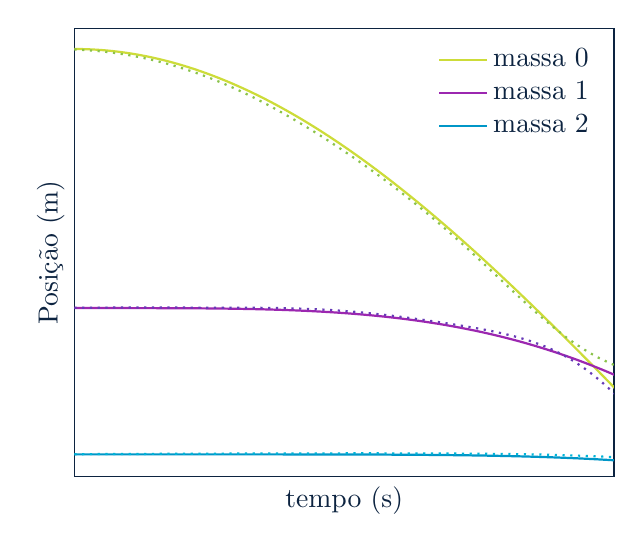
\begin{tikzpicture}
		\begin{axis}[
			%height=3.5cm,
			%width=\textwidth,
			domain=0:0.5,
			xmin=0,
			xmax=0.4,
               		legend style={fill=white,draw=none},
               		legend cell align={left},
               		%legend pos=outer north east,
			xlabel=\textcolor{UBI}{tempo $(\unit{\second})$},
			ytick={},
			yticklabels={},
			xtick={},
			xticklabels={},
			ymax=2.57,
			ymin=0,
			ylabel=\textcolor{UBI}{Posição $(\unit{\metre})$},
			%grid=both,
			major grid style={line width=.2pt,draw=pag!95},
			samples=400,
			ticks=none,
			%ylabel=,
			every axis/.append style={axis line style={UBI}, tick style={pag!80}}
			]
			
			\addplot[mylime, smooth, thick] {+2.4508266637798486+1.92551978e-06-7.08288771e-04*x-1.46868493e+01*x^2-4.09976421e-01*x^3+2.18585827e+01*x^4-9.39435949e+00*x^5-6.34499469e+00*x^6};
	\addlegendentry[UBI]{massa 0}	
			\addplot[mypurple, smooth, thick] {0.9655805946162642+5.849073753628633*x^6+16.602620664621227*x^5-23.992790391059497*x^4+0.721408292027056*x^3-0.049464418381870844*x^2+0.0012431133324992847*x-3.3748416628826994e-06};
           \addlegendentry[UBI]{massa 1}
			\addplot[p6, smooth, thick] {0.12706810953816955+0.49592093161308015*x^6-7.2082611722205305*x^5+2.1342076920531725*x^4-0.311431870599336*x^3+0.02131369465598449*x^2-0.0005348245618400737*x+1.449321886986526e-06};
           \addlegendentry[UBI]{massa 2}	
			
			\addplot[mylightgreen, dotted, thick] {2.45082666-5.52077707e-01*(x+0.05)+3.43475522e+01*(x+0.05)^2-7.74480255e+02*(x+0.05)^3+7.67559430e+03*(x+0.05)^4-4.78466157e+04*(x+0.05)^5+1.85156584e+05*(x+0.05)^6-4.25893494e+05*(x+0.05)^7+5.29402858e+05*(x+0.05)^8-2.72302397e+05*(x+0.05)^9};%lab
			
           
           
           
            %\addlegendentry[UBI]{Laboratorial (bola 1)}
			
			\addplot[mydeeppurple, dotted, thick] {+236878.24663477603*(x+0.05)^9-445940.6935199308*(x+0.05)^8+341684.85624595085*(x+0.05)^7-137516.49356955112*(x+0.05)^6+31308.952389044767*(x+0.05)^5-4064.7449218401653*(x+0.05)^4+286.3968820830498*(x+0.05)^3-9.702864113503072*(x+0.05)^2+0.14861681786073874*(x+0.05)+0.9655805946162642};%lab
          % \addlegendentry[UBI]{Laboratorial (bola 2)}
			
			\addplot[p5, dotted, thick] {+5919.067897122547*(x+0.05)^9-11617.379837153167*(x+0.05)^8+9381.76346394042*(x+0.05)^7-4036.0015719443286*(x+0.05)^6+992.5740054163633*(x+0.05)^5-138.15718216106012*(x+0.05)^4+9.591644806308794*(x+0.05)^3-0.1774404113040594*(x+0.05)^2+0.019261796302454434*(x+0.05)+0.12706810953816955};%lab
          % \addlegendentry[UBI]{Laboratorial (bola 3)}
		        
		\end{axis}
	\end{tikzpicture}
\end{document}